\documentclass[10pt,twocolumn]{article}

\usepackage{arxiv}
\usepackage[htt]{hyphenat}
\usepackage{amsmath,amssymb}
\usepackage{algorithm}
\usepackage[noend]{algpseudocode}

% Allow a little extra flexibility in paragraph justification so long \texttt
% identifiers (e.g. register_mask_sparse_device) don't trigger overfull hboxes.
\tolerance=2000
\emergencystretch=2em
\usepackage{booktabs}
\usepackage{tabularx}
\usepackage{array}
\usepackage{graphicx}
\usepackage{tikz}
\usetikzlibrary{arrows.meta,positioning,fit,backgrounds,calc,shapes.geometric}
\usepackage{listings}
\usepackage{xcolor}
\usepackage{caption}
\usepackage[hidelinks,colorlinks=true,
            linkcolor=black!70!blue,
            citecolor=black!70!blue,
            urlcolor=black!70!blue]{hyperref}
\usepackage[noabbrev,capitalise]{cleveref}
\crefname{algorithm}{Algorithm}{Algorithms}
\Crefname{algorithm}{Algorithm}{Algorithms}
\usepackage[backend=biber,style=numeric-comp,sorting=none]{biblatex}
\addbibresource{refs.bib}

\graphicspath{{figures/}}

% --- Listings: xlog + Python styles ---
\definecolor{codebg}{RGB}{248,248,248}
\definecolor{codekey}{RGB}{0,90,156}
\definecolor{codecomment}{RGB}{106,115,125}
\definecolor{codestring}{RGB}{163,21,21}

\lstdefinelanguage{xlog}{
  morekeywords={pred,func,domain,use,private,nn,true,false,not,and,or,if,then,else,is,query,fact,rule,count,sum,min,max,logsumexp,abs,pow,cast},
  sensitive=true,
  morecomment=[l]{//},
  morecomment=[s]{/*}{*/},
  morestring=[b]",
  literate={:-}{{{\color{codekey}:-}}}2
           {::}{{{\color{codekey}::}}}2
           {?-}{{{\color{codekey}?-}}}2
           {->}{{{\color{codekey}->}}}2
}
% Shared base style; xlog/python only override `language=`.
\lstdefinestyle{codebase}{
  backgroundcolor=\color{codebg},
  basicstyle=\ttfamily\small,
  keywordstyle=\color{codekey}\bfseries,
  commentstyle=\color{codecomment}\itshape,
  stringstyle=\color{codestring},
  frame=single,
  framerule=0.3pt,
  breaklines=true,
  breakatwhitespace=false,
  prebreak=\mbox{\textcolor{codecomment}{$\hookleftarrow$}},
  postbreak=\mbox{\textcolor{codecomment}{$\hookrightarrow$}\space},
  columns=fullflexible,
  showstringspaces=false,
  numbers=none,
  captionpos=b,
  abovecaptionskip=0.5em,
  belowcaptionskip=0.5em,
}
\lstdefinestyle{xlogstyle}{style=codebase,language=xlog}
\lstdefinestyle{pythonstyle}{style=codebase,language=Python}
\lstset{style=xlogstyle}

% Listings are referenced as "Listing N" via cleveref.
\crefname{lstlisting}{Listing}{Listings}
\Crefname{lstlisting}{Listing}{Listings}

% --- TikZ figure styles ---
\definecolor{figblue}{RGB}{0,90,156}
\definecolor{figgreen}{RGB}{27,128,79}
\definecolor{figgray}{RGB}{90,98,110}
\definecolor{figband}{RGB}{233,240,247}
\definecolor{figaccent}{RGB}{176,42,42}
\tikzset{
  fnode/.style={draw=figgray,rounded corners=2pt,fill=white,align=center,
                font=\small,inner sep=4pt,minimum height=8mm},
  fproc/.style={fnode,draw=figblue,very thick},
  fcert/.style={fnode,draw=figaccent,very thick},
  fneural/.style={fnode,draw=figgreen,very thick},
  flabel/.style={font=\scriptsize\itshape,figgray},
  farrow/.style={-{Stealth[length=2mm]},figgray,thick},
  fgrad/.style={-{Stealth[length=2mm]},figaccent,thick,dashed},
}

% --- Title block ---
\title{xlog: A Universal GPU-Native Engine for Neurosymbolic Integration}
\author{The xlog Project\\\small v0.9.2 Technical Whitepaper}
\date{June 2026}

\begin{document}
\twocolumn[
  \begin{@twocolumnfalse}
    \maketitle
    % Abstract — ported from docs/whitepaper-v050.md lines 5-8
\begin{abstract}
\noindent
% TODO(Task 3): port abstract content.
\end{abstract}

    \vspace{1.5em}
  \end{@twocolumnfalse}
]

\section{Introduction}\label{sec:intro}

Neurosymbolic systems combine neural perception with symbolic reasoning, but the two halves run on different machines. Deep learning frameworks---PyTorch, JAX---execute dense tensor computation on the GPU through optimized CUDA kernels. Logic engines---Datalog evaluators, probabilistic-logic systems such as ProbLog~\cite{problog2}, answer-set solvers---are CPU-bound interpreters and compilers. Every system that couples the two, from DeepProbLog~\cite{deepproblog} to NeurASP~\cite{neurasp}, therefore straddles the PCIe bus: each training iteration ships a network's outputs to a CPU logic engine, materializes query results or proofs, and pulls gradients back to update parameters. At scale---millions of ground atoms, thousands of steps---these host--device transfers, not the inference or learning itself, dominate wall-clock time and bandwidth.

The transfer wall is one half of the problem; partial coverage is the other. Existing neurosymbolic frameworks bridge a neural network to a \emph{single} symbolic backend---DeepProbLog to probabilistic logic, NeurASP to answer-set programming---and run that backend on the CPU. GPU logic efforts, conversely, accelerate one paradigm in isolation: deterministic Datalog~\cite{gpulog,vflog} or SAT~\cite{parafrost}, with no neural interface. No system makes the \emph{whole} symbolic spectrum---deterministic, probabilistic, and epistemic reasoning---both GPU-resident and differentiably coupled to neural networks.

xlog closes both gaps. It is a GPU-native logic programming language whose compiler and runtime treat a neural network as an ordinary predicate: the network's softmax output becomes a distribution over weighted facts that flow into whichever reasoning mode a program uses, and gradients flow back, all without leaving the device. Three mechanisms make this integration both universal and sound. A \emph{device-resident symbolic substrate} keeps fact stores, deltas, circuits, solver state, and gradient buffers in GPU memory throughout evaluation, so the symbolic half never crosses the bus. \emph{Verified knowledge compilation} turns a network's outputs into a differentiable arithmetic circuit and proves, on-device, that the circuit is logically equivalent to its source formula---so the neural--symbolic bridge is exact and machine-checked, not merely assumed. \emph{Zero-copy differentiable coupling} exports the resulting gradients through DLPack~\cite{dlpack} directly into PyTorch's autograd graph. The system is implemented in Rust with custom CUDA kernels organized into a layered crate architecture; host involvement is limited to orchestration, I/O, and compilation.

The principal contributions of this paper are:

\begin{itemize}
  \item \textbf{A universal neurosymbolic integration model.} A neural network is a predicate, and the same uniform, transfer-free mechanism connects it to deterministic, probabilistic, and epistemic reasoning---rather than a bespoke bridge to one backend (\Cref{sec:arch,sec:nesy}).
  \item \textbf{A GPU-resident symbolic substrate.} Semi-naive Datalog evaluation with stratified negation and aggregation runs as custom CUDA relational kernels, extended with a worst-case-optimal join (WCOJ) subsystem that avoids the intermediate-relation blowup of binary-join plans on skewed cyclic queries (a measured $27.96\times$ geometric-mean ablation, \Cref{sec:datalog}).
  \item \textbf{GPU-native verified knowledge compilation.} A provenance$\to$CNF$\to$D4$\to$circuit pipeline runs entirely on device, and an on-GPU CDCL solver proves each compiled circuit equivalent to its source formula. To our knowledge this is the first end-to-end GPU-resident knowledge-compilation pipeline with on-device equivalence verification, and it is the paper's central technical result (\Cref{sec:prob}).
  \item \textbf{End-to-end differentiable training with zero-copy interop.} Compiled circuits are cached across iterations and evaluated as level-parallel forward/backward kernels, with gradients exported zero-copy via DLPack and Arrow; circuit caching yields a measured $2.74\times$ training speedup. Term embeddings and differentiable ILP ride the same device-resident path (\Cref{sec:nesy}).
  \item \textbf{Full-spectrum reach.} Epistemic reasoning over world views (\texttt{know}/\texttt{possible} under founded and Gelfond-style semantics) and well-founded semantics execute on the same substrate, reusing the CDCL, join, and circuit machinery rather than a separate engine (\Cref{sec:epistemic}).
\end{itemize}

The remainder of this paper is organized as follows. \Cref{sec:arch} presents the integration model and system architecture. \Cref{sec:lang} describes the xlog language. \Cref{sec:datalog} details the GPU-resident symbolic substrate. \Cref{sec:prob} presents verified knowledge compilation, the central contribution. \Cref{sec:nesy} ties the pieces together as end-to-end neurosymbolic learning. \Cref{sec:epistemic} extends the substrate to epistemic and other reasoning modes. \Cref{sec:eval} reports evaluation results, \Cref{sec:related} surveys related work, and \Cref{sec:limits} discusses limitations and future work.

\section{Architecture}\label{sec:arch}
% TODO(Task 4): port Section 2 from docs/whitepaper-v050.md lines 31-111.

\section{The xlog Language}\label{sec:lang}

This section describes the xlog language surface: types, expressions, user-defined functions, modules, and stratified aggregations with constraints. Probabilistic facts (\texttt{p::f.}) and neural predicate declarations (\texttt{nn/k}) are language-level constructs described in \Cref{sec:prob} and \Cref{sec:nesy} respectively.

\subsection{Design Philosophy}\label{sec:lang:philosophy}

\subsection{Type System}\label{sec:lang:types}

\subsection{Expressions and Arithmetic}\label{sec:lang:arith}

\subsection{User-Defined Functions}\label{sec:lang:udf}

\subsection{Modules and Imports}\label{sec:lang:modules}

\subsection{Aggregations and Constraints}\label{sec:lang:agg}

\section{GPU-Native Datalog Evaluation}\label{sec:datalog}

\Cref{sec:lang} describes the source language; this section describes how its Datalog subset compiles to and executes on the GPU. The deterministic evaluation engine executes standard Datalog with stratified negation and aggregation entirely on the GPU. The algorithmic approach---semi-naive fixpoint iteration over stratified programs---is well established. The contribution here is not algorithmic novelty but engineering: every relational operator runs as a custom CUDA kernel, delta relations are maintained on-device, and no host--device transfers occur during evaluation.

\subsection{Semi-Naive Evaluation on GPU}

The executor in \texttt{crates/xlog-runtime/src/executor/} processes an \texttt{ExecutionPlan} consisting of strata ordered by the dependency analysis from \Cref{sec:arch}. Each stratum contains one or more strongly connected components (SCCs), and the executor dispatches each SCC according to whether it is recursive or non-recursive.

\textbf{Non-recursive SCCs.} The executor evaluates each compiled rule once, passing the RIR tree to the node dispatcher which invokes the appropriate CUDA kernel for each operator (scan, join, filter, project, group-by). Results for the same head predicate are merged via the \texttt{union\_gpu} kernel and deduplicated. No iteration is needed.

\textbf{Recursive SCCs.} The \texttt{execute\_recursive\_scc} method in \texttt{crates/xlog-runtime/src/executor/recursive.rs} implements semi-naive evaluation. The algorithm proceeds in three phases:

\begin{enumerate}
  \item \textbf{Seeding.} Every rule in the SCC is evaluated once against the current relation store, and each predicate's initial delta is the set difference between the newly derived tuples and any pre-existing ones. Delta relations are distinct on-device buffers.
  \item \textbf{Iteration.} Each rule is re-evaluated through delta-rewritten variants---one variant per recursive scan occurrence, so self-joins are handled correctly: a body containing \texttt{p(X,Y), p(Y,Z)} yields two variants, each substituting the delta into exactly one scan. Variant results are unioned per head predicate, differenced against the full relation, and deduplicated, all on-device. When no predicate produces new tuples, the fixpoint is reached.
  \item \textbf{Merge and cleanup.} New delta tuples are merged into the full relation by union and sorted deduplication. At fixpoint---or when the iteration cap (default 1{,}000{,}000) is hit---delta relations are freed.
\end{enumerate}

All intermediate buffers remain on-device throughout. The profiler records per-operator timing, row counts, and peak memory, feeding the optimizer loop described below.

\subsection{Kernel Design}

xlog implements its relational algebra as eight direct CUDA kernels rather than wrappers over cuBLAS, cuSPARSE, or Thrust. The reason is the residency contract: a library operator imposes its own allocation, synchronization, and host-staging behavior, which would defeat the zero-transfer guarantee of \Cref{sec:arch}. Bespoke kernels keep every intermediate buffer on-device and let every launch flow through the recorded-launch discipline. \Cref{tab:kernels} summarizes them; the worst-case-optimal multiway join described below is a ninth kernel family.

\begin{table}[htbp]
  \centering
  \caption{Core relational CUDA kernels in \texttt{xlog-cuda}.}
  \label{tab:kernels}
  \small
  \begin{tabularx}{\linewidth}{@{}l X@{}}
    \toprule
    \textbf{Kernel} & \textbf{Purpose} \\
    \midrule
    \texttt{join.cu}    & Hash join with linked-list collision chains and FNV-1a composite hashing over raw key bytes, so all scalar types share one path. Includes count\,$\to$\,scan\,$\to$\,materialize (CSM) variants for Inner and LeftOuter joins. \\
    \texttt{sort.cu}    & Stable 4-bit radix sort (8 passes over 32-bit keys): per-pass histogram, prefix sum, scatter. \\
    \texttt{filter.cu}  & Comparison operators for column-vs-constant and column-vs-column, with stream compaction via prefix sum and fused compare-and-scan variants. \\
    \texttt{groupby.cu} & Sorted-input grouped aggregation: boundary detection in sorted keys, then per-group Count/Sum/Min/Max/LogSumExp reduction. \\
    \texttt{dedup.cu}   & Sort-based deduplication and set difference with type-aware equality, including IEEE~754 float handling. \\
    \texttt{set\_ops.cu} & Union (concat\,+\,sort\,+\,dedup) and set difference via sorted-array binary search. \\
    \texttt{scan.cu}    & Blelloch parallel prefix sum---the building block for filter compaction, dedup, and group-by. \\
    \texttt{pack.cu}    & Multi-column key packing into row-major byte arrays with FNV-1a hashing, eliminating host roundtrips for join-key preparation. \\
    \bottomrule
  \end{tabularx}
\end{table}

Every operator also exposes a recorded-launch sibling (since v0.6.0) that routes through the \texttt{LaunchRecorder} preflight/commit discipline of \Cref{sec:arch}, selectable per-operator or via an umbrella flag, with the legacy path as the default.

\textbf{IEEE~754 total ordering.} The filter kernel implements a correctness-critical design choice for floating-point comparisons. Equality and inequality (Eq, Ne) use standard IEEE~754 semantics where $\mathrm{NaN} \neq \mathrm{NaN}$. Ordered comparisons (Lt, Le, Gt, Ge) use a total ordering transformation: the \texttt{float\_to\_ordered\_f64} device function converts an \texttt{f64} bit pattern to an \texttt{i64} such that the resulting integer order matches the IEEE~754 \texttt{totalOrder} predicate. The ordering is: $-\mathrm{NaN} < -\mathrm{Inf} <$ negative finites $< -0.0 < +0.0 <$ positive finites $< +\mathrm{Inf} < +\mathrm{NaN}$. The transformation works by flipping all bits except the sign bit for negative values and flipping only the sign bit for non-negative values, matching Rust's \texttt{f64::total\_cmp()} algorithm. An analogous \texttt{float\_to\_ordered\_f32} function handles 32-bit floats. This ensures that Datalog programs produce deterministic, well-defined results for all floating-point inputs, including edge cases involving NaN and signed zeros.

\subsection{Adaptive Join Planning}

The optimizer performs cost-based query transformations using runtime statistics collected during prior executions.

\textbf{Cost model.} Each plan node is costed along four dimensions---expected row count, CPU coordination cost, peak GPU memory, and number of host--device transfers---with transfers penalized heavily to reflect PCIe latency. The transfer penalty is what makes the planner prefer device-resident plans even when they cost more raw compute.

\textbf{Predicate pushdown.} When enabled (the default), the optimizer pushes \texttt{Filter} nodes below \texttt{Project} and \texttt{Join} nodes. Filters above joins are decomposed: predicates referencing only left-side columns are pushed into the left input, predicates referencing only right-side columns into the right input, and cross-predicates remain above the join. Filters above projections are remapped through pass-through columns where possible.

\textbf{Join ordering.} For queries of up to ten relations the optimizer uses dynamic programming to select the minimum-cost join order; above that threshold it falls back to a greedy heuristic to avoid exponential planning time. Cardinality estimates multiply left and right cardinalities by a selectivity factor learned from prior executions.

\textbf{Feedback loop.} The executor can export a statistics snapshot---per-relation cardinality, byte size, access heat, column statistics, and join selectivities---and merge it back before the next compilation, closing the loop between execution and optimization. A predicate-name mapping keeps these statistics valid across compilations even when internal relation IDs are reassigned.

\subsection{Worst-Case Optimal Joins}

Binary-join plans can materialize intermediate relations that are asymptotically larger than the final result---the classic pathology for cyclic queries such as triangle enumeration. This is not a corner case for the Datalog workloads xlog targets: program-analysis queries (points-to analysis, call-graph and reachability inference over code-dependency graphs) are dominated by cyclic, skewed join patterns where the intermediate blowup, not the final answer, governs cost. xlog addresses this with a worst-case-optimal join (WCOJ) subsystem~\cite{ngo2018wcoj,veldhuizen2014leapfrog,wang2023freejoin}. A pure-Rust hypergraph planner (\texttt{xlog-logic::hypergraph}) analyzes rule bodies for multiway-join eligibility, derives a deterministic variable ordering from cardinality and selectivity statistics, and emits a \texttt{MultiWayJoin}/\texttt{ChainJoin} RIR node when promotion provably preserves output semantics; otherwise the binary-join plan is retained as a certified fallback. Planner verdicts and GPU outputs are certified against the same CPU oracle fixtures before executor wiring.

The GPU side (\texttt{wcoj.cu}, 2{,}262 LOC) executes the join via count $\to$ device-side prefix scan $\to$ materialize over flat sorted-column storage, with a four-byte metadata D2H total and no count-vector transfer. A sorted-layout fast path proves already-sorted-and-unique inputs with a recorded checker kernel and clones on-device instead of re-sorting. Coverage extends from the canonical triangle to 4-cycles, K-clique templates (K${=}5$--$8$), recursive/SCC integration, and helper-relation splitting that exposes inner skew to root-level histograms.

A default-on adaptive skew classifier decides per query whether to dispatch WCOJ: high-skew inputs take the WCOJ path while uniform or empty inputs fall back to the binary-join chain. \texttt{XLOG\_DISABLE\_WCOJ\_TRIANGLE=1} is the hard kill switch. \Cref{sec:eval} reports the measured speedup envelope on skewed paper-scale workloads.

\subsection{Runtime Optimization Layer}

Interactive and long-running deployments---REPL sessions, iterative solver loops, incremental ML training---repeatedly evaluate similar queries over relations that change little between calls. A stateless executor rebuilds join indices and recomputes shared subplans on every call, paying the dominant cost each time. v0.8.6 adds three runtime optimizations that exploit this between-call stability, each with explicit off/on controls and zero added data-plane host transfers. \emph{Common-subexpression elimination} caches the results of safe deterministic subplans within an evaluation, invalidated on relation-generation change, removing duplicate work. \emph{Adaptive re-optimization} lets the executor adopt a compiler-supplied candidate plan (via \texttt{execute\_plan\_with\_adaptive\_candidate}) when deterministic mis-plan telemetry crosses a configurable ratio, with GPU output equivalence and rollback diagnostics. A \emph{persistent hash-index manager}, keyed on relation generation, schema, and device, retains built indices across repeated session evaluations with deterministic LRU eviction and background-build accounting; on a build-heavy repeated-session fixture it records a $3.21\times$ speedup against a $1.5\times$ target with zero tracked host transfers (\Cref{sec:eval}). Persistent sessions additionally coalesce relation-delta batches and expose opt-in, metadata-only relation-change callbacks.

\subsection{Reversible Symbols}

Datalog programs operate on strings, but GPU kernels operate on fixed-width numeric columns. xlog bridges this with a global symbol table that interns each unique string to a dense, sequential \texttt{u32} identifier and resolves it back in $O(1)$ at output time. Dense zero-based IDs give GPU-friendly access patterns, and symbol columns then \emph{are} ordinary \texttt{u32} columns---join, sort, filter, and dedup kernels operate on them with no special-casing. The table itself stays host-side, since variable-length string data is needed only at ingestion and output boundaries. The \texttt{symbol} type maps to Arrow's \texttt{Dictionary(UInt32, Utf8)}, so export to Arrow consumers (cuDF, Polars, DuckDB) is zero-copy while preserving the compact internal representation.

\section{Probabilistic Inference on GPU}\label{sec:prob}

\subsection{Approach}

Probabilistic logic programming systems such as ProbLog~\cite{problog2} compute the probability of queries over programs containing probabilistic facts. The standard technique is knowledge compilation: compile the ground Boolean formula derived from provenance tracking into a tractable circuit (typically a Decision-DNNF), then evaluate weighted model counts over that circuit. ProbLog follows a compile-once/evaluate-many model: the circuit structure is determined by the logical program and is independent of the probability weights, so a single compilation can serve many weight configurations during parameter learning.

xlog adopts the same compile-once/evaluate-many model but moves the entire pipeline onto the GPU. In ProbLog, provenance extraction, CNF encoding, D4 compilation, and circuit evaluation all execute on the CPU. When ProbLog is paired with a neural component (as in DeepProbLog~\cite{deepproblog}), each training iteration requires transferring circuit evaluation results from CPU to GPU for gradient computation, and pulling gradients back for weight updates. xlog eliminates this architectural split: PIR extraction, Tseitin~\cite{tseitin} CNF encoding, D4~\cite{d4compiler} compilation, CDCL equivalence verification, and forward/backward circuit evaluation all execute as CUDA kernels on the GPU. The compiled circuit is a GPU-resident data structure (XGCF), weight buffers and gradient buffers are GPU-resident, and no host--device transfers occur in the evaluation hot path. This design turns what would be a PCIe-bottlenecked ping-pong between CPU logic engine and GPU tensor framework into a single-device pipeline.

\subsection{GPU Knowledge Compilation Pipeline}

The probabilistic compilation pipeline transforms a Datalog program with probabilistic annotations into a GPU-resident arithmetic circuit through five stages (\Cref{fig:kc}). Each stage is implemented as one or more CUDA kernel launches, with intermediate data structures remaining in device memory throughout.

\begin{figure}[htbp]
  \centering
  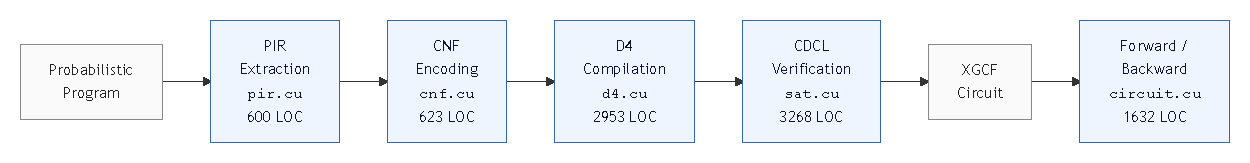
\includegraphics[width=\linewidth]{kc_pipeline.pdf}
  \caption{Knowledge compilation pipeline. All five stages execute as CUDA kernels on GPU-resident data; no host--device transfers occur between stages.}
  \label{fig:kc}
\end{figure}

The five stages map to the kernel files \texttt{pir.cu}, \texttt{cnf.cu}, \texttt{d4.cu}, \texttt{sat.cu}, and \texttt{circuit.cu}.

\textbf{Stage 1: PIR extraction.} Provenance tracking over deterministic evaluation produces a weighted Boolean formula. The interner hash-conses node batches on the GPU, deduplicating structurally identical subformulas through an atomic GPU hash table. This on-device deduplication is essential: grounding can produce exponentially many redundant subformulas, and interning on the host would force the full uninterned graph into host memory---reintroducing the very transfer the pipeline exists to avoid.

\textbf{Stage 2: CNF encoding.} A Tseitin transformation lowers the formula to CNF entirely on GPU, using parallel prefix sums to assign compact, gap-free variable IDs and emit clauses into a device-resident compressed-sparse-row structure.

\textbf{Stage 3: D4 compilation.} The most complex stage compiles the CNF into a Decision-DNNF circuit (the XGCF format) via a GPU-native variant of the D4 algorithm~\cite{d4compiler}. A BFS frontier exposes parallelism, then per-block DFS workers perform component detection, decision-variable selection via VSIDS-like activity scores~\cite{grasp}, and recursive decomposition. A smoothing pass forces every branch of an OR/Decision node to mention the same variable set---required for correct weighted model counting---and the result is levelized so each topological level evaluates in one kernel launch.

\textbf{Stage 4: CDCL verification.} Rather than trust the compiler, xlog proves the compiled circuit $C$ is equivalent to the source formula $\varphi$: it solves $\varphi \land \lnot C$ and $C \land \lnot \varphi$ on a GPU CDCL solver, both of which must be unsatisfiable. This is a complete formal proof, not a sampling check. UNSAT results carry a resolution proof checked on-device, and the solver never reads its status back to the host---a wrong answer triggers a device-side trap. Circuit correctness thus becomes a machine-checked certificate rather than an assumption, which matters because a silently miscompiled circuit would corrupt every downstream probability and gradient.

\textbf{Stage 5: circuit evaluation.} The verified XGCF supports a level-parallel forward pass (log-space weighted model counting, one kernel per level, yielding $\log Z$) and a reverse-order backward pass that accumulates per-variable gradients. Both leave their results in GPU-resident buffers consumable directly by PyTorch via DLPack (\Cref{sec:nesy}).

\subsection{Circuit Caching}

D4 compilation is the most expensive stage in the pipeline. On the MNIST addition benchmark (\texttt{01\_minimal}, 512 training examples), a cold-start compilation takes approximately 75 seconds. Since this cost is incurred at the beginning of each training epoch in a naive implementation, it can dominate total training time.

The key insight enabling circuit caching is that the XGCF circuit structure depends on the logic program---specifically, on the propositional structure of the grounded rules and the evidence pattern---but not on the numerical values of the probability weights. When neural network parameters change between training iterations, the weights assigned to probabilistic facts change, but the Boolean formula and its compiled Decision-DNNF structure remain identical. This means the compiled XGCF can be cached and reused across all training iterations, with only the weight buffers updated before each forward pass.

The \texttt{GpuCircuitCache} in \texttt{crates/xlog-prob/src/compilation/gpu\_cache.rs} implements this caching. On the first evaluation, the full pipeline runs (PIR extraction, CNF encoding, D4 compilation, CDCL verification), and the resulting \texttt{GpuXgcf} is stored in the cache keyed by a structural hash of the PIR graph and evidence configuration. On subsequent evaluations, the cache returns the existing circuit, and only the weight-upload and forward/backward passes execute. The cache also stores the CNF variable tables (\texttt{GpuCnfVarTables}) needed to map between PIR leaf IDs and CNF variable IDs for weight construction.

Measured impact: on the MNIST addition benchmark (3 epochs, 512 training examples, 3 seeds), cache-enabled training completes in a mean of $88.89$ seconds (std: $3.48$\,s), compared to $242.90$ seconds (std: $8.19$\,s) with caching disabled. This yields a $2.74\times$ end-to-end speedup (95\% CI: $[2.29, 3.18]$). The speedup is large because D4 compilation cost is amortized across all epochs: in the latest checked-in post-fix rerun on \texttt{main}, the first epoch averages $71.654$\,s while warm epochs average $0.248$\,s once the cached circuit and batched evaluation path are active (\Cref{sec:eval}).

\subsection{Monte Carlo Sampling}

For programs where exact inference via knowledge compilation is infeasible---either because the ground formula is too large for D4 compilation within the available GPU memory, or because the user prefers approximate results with bounded computation---xlog provides a GPU-parallel Monte Carlo sampling engine implemented in \texttt{crates/xlog-prob/src/mc/}.

The MC engine supports two sampling methods, selectable via \texttt{McSamplingMethod}:

\begin{itemize}
  \item \textbf{Rejection sampling.} The sampler draws values for all probabilistic facts from their prior distributions on the GPU, then evaluates the deterministic Datalog program in each sampled world. Worlds where the evidence is not satisfied are discarded. Query probabilities are estimated as the fraction of accepted worlds in which each query atom is derived. This method is unbiased but can be inefficient when the evidence has low prior probability, as most samples are rejected.
  \item \textbf{Evidence clamping.} When all evidence atoms correspond to Bernoulli probabilistic facts, the sampler can force those facts to their observed values, guaranteeing that every sample satisfies the evidence. This eliminates rejection waste entirely: the \texttt{McCountStrategy} switches to \texttt{QueriesOnly} mode, skipping evidence-side buffer allocations and truth-kernel evidence checks. Evidence clamping is auto-selected when the \texttt{EvidenceForcing} analysis determines that all evidence is forceable (i.e., each evidence atom maps to a single probabilistic fact with no intermediate rules).
\end{itemize}

Both methods report confidence intervals for estimated probabilities. The sampling loop is structured to minimize per-sample overhead: probabilistic fact values are sampled in bulk on the GPU via the \texttt{sampling} submodule, the relation store is reset using a targeted \texttt{McSampleResetPlan} that preserves pure deterministic relations and clears only dynamic relations (avoiding a full store clone per sample), and per-sample pointer buffers are pre-allocated outside the sample loop. The current repository contains these hot-loop optimizations in code, but does not ship a standalone archived MC timing report with stable phase-by-phase numbers, so this paper limits itself to the implementation strategy rather than quoting unsupported per-benchmark deltas.

\subsection{Probabilistic Aggregates}

v0.8.5 extends probabilistic inference with finite aggregate queries. Aggregate heads and outputs over \texttt{count}, \texttt{sum}, \texttt{min}, \texttt{max}, and \texttt{logsumexp} are evaluated in both exact provenance/PIR inference and Monte Carlo deterministic aggregate execution, subject to a typed exact-domain cap that rejects domains too large for tractable enumeration (with a diagnostic recommending MC or a smaller finite domain). For small finite \texttt{count} domains, \emph{aggregate lifting} replaces naive world enumeration with exact cardinality dynamic programming over a compact state set---collapsing, for example, a $2^{17}$-outcome enumeration into roughly $170$ lifted states with identical results. Accepted fired \texttt{count} aggregate queries dispatch a GPU-native exact evaluator (\texttt{weights\_count\_lift\_exact}) rather than a CPU finite-world shortcut, keeping the exact aggregate path device-resident; explain metadata records which aggregate operators fired versus fell back to exact enumeration.

\subsection{Well-Founded Semantics}

Standard stratified negation requires that no recursive cycle passes through a negated literal. Programs that violate this constraint---such as the classic \texttt{p :- not q.\ q :- not p.}---have no two-valued stable model and are rejected by most Datalog engines. xlog handles such non-monotone programs via Well-Founded Semantics (WFS), implemented in \texttt{crates/xlog-prob/src/wfs.rs}.

WFS assigns three-valued truth to atoms: true, false, or undefined. The algorithm computes an alternating fixed point: (1) find the greatest unfounded set (atoms that cannot be supported by any rule), mark them false; (2) derive all consequences of the current knowledge, mark them true; (3) repeat until stable. Atoms that remain neither true nor false are classified as undefined. For probabilistic programs, true atoms receive normal probability and gradient computation, while false and undefined atoms are assigned probability zero with zero gradients---matching ProbLog's conservative treatment of non-stratified programs.

WFS is invoked automatically during provenance extraction when a non-monotone SCC is detected. The Monte Carlo engine, by contrast, is the GPU-resident Datalog megakernel (\texttt{crates/xlog-prob/src/mc/resident.rs}): it evaluates every sampled world in a single device launch with a device-side bounded fixpoint and supports only \emph{bounded-domain positive} Datalog (arity $\leq 2$, body $\leq 2$). Non-monotone and otherwise unsupported fragments are \emph{rejected fail-closed} before execution with a typed diagnostic (there is no host-orchestrated fallback); such programs must use the exact / WFS path. A representative supported MC program is \texttt{examples/prob/04-recursive-mc.xlog}, a recursive transitive closure (\texttt{reach(X,Z) :- reach(X,Y), edge(Y,Z).}) whose non-base tuple \texttt{reach(1,3)} is derived by a multi-iteration device-side fixpoint.

\section{Neurosymbolic Integration}\label{sec:nesy}

This section is where the three pillars meet. The device-resident substrate (\Cref{sec:datalog}) keeps the symbolic state on the GPU; verified knowledge compilation (\Cref{sec:prob}) turns a network's outputs into a sound differentiable circuit; and zero-copy coupling carries gradients back into the neural optimizer without leaving the device. Together they let neural perception and logical reasoning train jointly, end to end, with no host--device transfers in the loop.

\subsection{Neural Predicates}

In xlog a neural network \emph{is} a predicate. The \texttt{nn/4} declaration embeds a network directly into the program:

\begin{lstlisting}[style=xlogstyle,
                   caption={Neural predicate declaration (\texttt{nn/4}).},
                   label={lst:nn-decl}]
nn(network_name, [input_vars], output_var,
   [output_labels]) :: predicate(args).
\end{lstlisting}

This is not a foreign-function escape hatch: it states that evaluating \texttt{predicate(args)} requires a forward pass through the named network, whose softmax over the label set becomes a distribution over probabilistic facts feeding the knowledge-compilation pipeline of \Cref{sec:prob}. On the Python side a PyTorch module is registered against the predicate:

\begin{lstlisting}[style=pythonstyle,
                   caption={Registering a PyTorch module against a neural predicate.},
                   label={lst:nn-register}]
program.register_network("mnist_net", net, optimizer)
\end{lstlisting}

The dataflow runs in two directions. \textbf{Forward:} when evaluation reaches an \texttt{nn/4}-backed predicate, the registered module runs, and its softmax vector is decomposed into weighted probabilistic facts---one per label---fed into the PIR/CNF/D4/XGCF pipeline. Because circuit structure depends on the program, not the weights, the compiled circuit is cached and only the leaf weights are updated on later iterations. \textbf{Backward:} after the circuit computes the forward log-probability and backward gradients via level-parallel kernels, the per-leaf gradient buffers are exported as DLPack tensors and injected into PyTorch's autograd graph, and the optimizer updates the network as usual. The GIL is released during GPU work, so CUDA execution does not block the interpreter.

\subsection{End-to-End Training}

The canonical example is MNIST addition (the DeepProbLog benchmark): given two digit images, predict their sum, with supervision only on sums---the network never sees individual digit labels. The entire reasoning structure is two rules:

\begin{lstlisting}[style=xlogstyle,
                   caption={MNIST addition: a CNN-backed digit predicate and an addition rule.},
                   label={lst:mnist-prog}]
nn(mnist_net, [X], Y, [0,1,2,3,4,5,6,7,8,9])
    :: digit(X, Y).
addition(X, Y, Z) :-
    digit(X, D1), digit(Y, D2), Z is D1 + D2.
\end{lstlisting}

The \texttt{nn/4} declaration connects the CNN to \texttt{digit/2}; the addition rule computes every consistent decomposition of a sum through probabilistic marginalization. Each query \texttt{addition(i, j, s)} trains by minimizing $-\log P(\texttt{addition}(i, j, s))$ under the compiled circuit. The driver compiles the program, registers the network, and runs the loop, which batches queries sharing a circuit template and runs forward/backward over the cached circuit:

\begin{lstlisting}[style=pythonstyle,
                   caption={Python driver: compile, register, train.},
                   label={lst:mnist-train}]
program = pyxlog.Program.compile(SRC)
program.register_network("mnist_net", net, optimizer)
program.add_tensor_source("train", train_images)
history = pyxlog.train_model_tensor(
    program, queries,
    epochs=epochs, batch_size=batch_size)
\end{lstlisting}

\begin{figure*}[tbp]
  \centering
  \resizebox{0.86\linewidth}{!}{%
  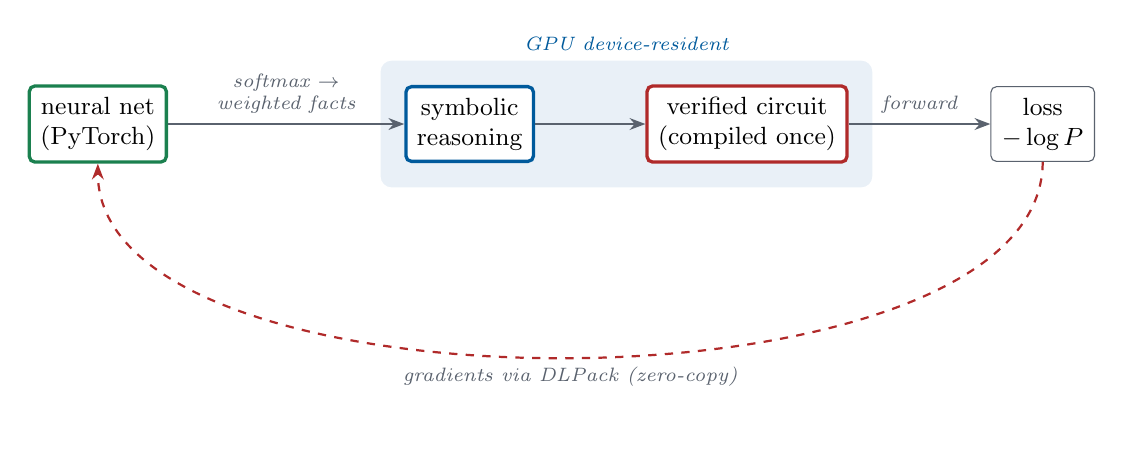
\begin{tikzpicture}
    \node[fneural] (net) {neural net\\(PyTorch)};
    \node[fproc,right=30mm of net] (sym) {symbolic\\reasoning};
    \node[fcert,right=14mm of sym] (circ) {verified circuit\\(compiled once)};
    \node[fnode,right=18mm of circ] (loss) {loss\\$-\log P$};
    \draw[farrow] (net) -- node[flabel,above,align=center]{softmax $\to$\\weighted facts} (sym);
    \draw[farrow] (sym) -- (circ);
    \draw[farrow] (circ) -- node[flabel,above]{forward} (loss);
    \draw[fgrad] (loss.south) to[out=-90,in=-90,looseness=0.7]
          node[flabel,below]{gradients via DLPack (zero-copy)} (net.south);
    \begin{scope}[on background layer]
      \node[fill=figband,rounded corners,fit=(sym)(circ),inner sep=3mm] (band) {};
    \end{scope}
    \node[flabel,figblue,anchor=south] at (band.north) {GPU device-resident};
  \end{tikzpicture}}
  \caption{One end-to-end neurosymbolic iteration, exhibiting the three pillars: a device-resident symbolic substrate (the shaded region never leaves the GPU), verified knowledge compilation (the circuit is compiled and proven correct once, then reused), and zero-copy differentiable coupling (gradients return through DLPack into PyTorch's autograd graph).}
  \label{fig:training}
\end{figure*}

The decisive performance property (\Cref{fig:training}) is that compilation and verification happen once, on the first forward pass; every later iteration reuses the cached circuit, executing only the weight update and the level-parallel forward/backward kernels. This is the mechanism behind the $2.74\times$ training speedup; the loss reduction across seeds confirms that gradients flow from circuit evaluation through the logic program back to the CNN, and the full timing breakdown is reported in \Cref{sec:eval}.

\subsection{Zero-Copy Interoperability}\label{subsec:interop}

A GPU-native engine is only useful if results reach the frameworks researchers already use---without copies that would reintroduce the transfer wall. xlog exposes its device-resident state through four standard interfaces.

\textbf{DLPack.} Each relation column or gradient buffer becomes a managed DLPack~\cite{dlpack} tensor whose GPU memory is reference-counted and freed only when every consumer releases it; on import, xlog validates device, dtype, contiguity, and alignment, optionally against an expected schema. In Python the protocol surfaces as a capsule, so \texttt{torch.from\_dlpack} yields a live CUDA tensor backed by the very memory xlog wrote.

\textbf{Arrow.} For columnar tools (Polars, DuckDB, cuDF), relations export through the Arrow~\cite{arrow} C Device Data Interface; symbol columns export as Arrow dictionary arrays, so a consumer reads symbolic columns as native string dictionaries while xlog keeps the compact integer representation.

\textbf{Python bindings.} The \texttt{pyxlog} extension (PyO3~\cite{pyo3}) exposes compilation, evaluation, training, and result extraction; tensor-valued results are returned as DLPack capsules, and long-running GPU operations release the GIL so data-loader threads proceed concurrently.

\textbf{PyTorch autograd.} The circuit behaves as a differentiable function inside PyTorch: the network's grad-enabled forward feeds the circuit, the scalar loss is exported via DLPack and re-imported, and a batched path stacks inputs into one forward pass and runs a single backward---so gradients flow from the logic layer back to \texttt{nn.Module} parameters with no custom autograd \texttt{Function}.

\subsection{Term Embeddings and Differentiable ILP}

Two further paths ride the same device-resident bridge. \textbf{Term embeddings} attach dense, optionally trainable vectors to logical symbols: where \texttt{nn/4} maps perception to discrete facts, embeddings give logical entities a continuous representation that participates in neural computation, with gradients flowing through the embedding lookup---enabling, for example, knowledge-graph entity representations trained jointly with neural perception. \textbf{Differentiable ILP} learns first-order rules rather than network weights: candidate rules are represented as sparse bitmasks over the ground-atom space, credit assignment runs entirely on-device via scatter--gather, and a six-gate promotion pipeline (convergence, novel-rate, regression, held-out F1, ambiguity, typed-schema checks) controls which rules are committed. This sparse, GPU-resident formulation avoids the cubic blowup of dense rule materialization; it is a beta subsystem (\Cref{sec:limits}).

\input{sections/07_epistemic.tex}
\section{Evaluation}\label{sec:eval}

This section reports artifact-backed measurements for xlog's deterministic, probabilistic, and neural-symbolic subsystems. Every quantitative claim is tied to a checked-in benchmark artifact. \emph{These are single-system measurements on development hardware: ablations of xlog against xlog's own baselines, not controlled head-to-head comparisons against other engines} (\Cref{sec:limits}). Throughput-target envelopes for operations measured only in isolation are maintained as an internal regression contract and are not restated here.

\subsection{Methodology}

All measurements were collected on an NVIDIA RTX PRO 3000 (Blackwell, 12\,GB VRAM, compute capability 12.0). Rust crates are built in release mode; CUDA modules are staged cubin-first with PTX fallback and explicit JIT warm-up; Python components use \texttt{pyxlog} with CUDA-enabled PyTorch. The benchmark harness uses Criterion.rs with the settings in \Cref{tab:stat-protocol}, and GPU measurements include warm-up to amortize kernel-module loading and CUDA context setup.

\begin{table}[htbp]
  \centering
  \caption{Benchmark harness settings.}
  \label{tab:stat-protocol}
  \small
  \begin{tabular}{@{}ll@{}}
    \toprule
    \textbf{Setting} & \textbf{Value} \\
    \midrule
    Sample size       & 10--100 runs (benchmark-dependent) \\
    Warm-up           & 3 iterations (PTX JIT, memory-pool init) \\
    Significance level & 0.10 \\
    Noise threshold   & 0.05 (ignore ${<}5\%$ variance) \\
    Seeding           & Deterministic LCG \\
    \bottomrule
  \end{tabular}
\end{table}

\subsection{Worst-Case Optimal Joins}

The WCOJ subsystem (\Cref{sec:datalog}) is measured against the binary-join baseline on four paper-scale fixtures---call-graph edges, Andersen points-to~\cite{andersen1994}, \texttt{ddisasm}-style disassembly~\cite{ddisasm}, and a recursive neural-symbolic mining analog---each with $4.19$M input rows. We measure at this scale deliberately: WCOJ speedups depend strongly on input size and skew, and synthetic micro-benchmarks systematically overstate them, so multi-rule recursive workloads at millions of tuples are the honest setting. Both paths must produce identical row sets before timing, and every measurement is a median over 10 runs with coefficient of variation ${\le}0.05$.

\Cref{fig:wcoj} reports the speedups: a $27.96\times$ geometric mean, with every fixture between $26.6\times$ and $29.6\times$.

\begin{figure}[htbp]
  \centering
  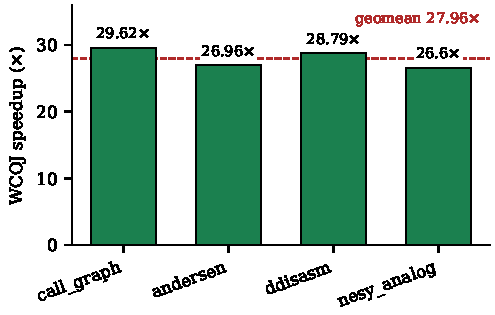
\includegraphics{results.pdf}
  \caption{WCOJ vs.\ binary-join speedup on four paper-scale fixtures ($4.19$M input rows each). Single-system ablation; the dashed line is the geometric mean.}
  \label{fig:wcoj}
\end{figure}

On uniform or empty inputs the adaptive classifier falls back to the binary-join chain. Peak observed allocation was about $2.3$\,GB, within the device's 12\,GB budget.

\subsection{Circuit Caching and Training}

Neural-symbolic training is measured on MNIST single-digit addition (512 training images, 5 epochs, batch size 64). Circuit caching (\Cref{sec:prob}) amortizes D4 compilation across epochs: a cache ablation over 3 seeds and 3 epochs reduced mean training time from $242.9$\,s (uncached) to $88.9$\,s (cached), a $2.74\times$ speedup (95\% CI $[2.29, 3.18]$). \Cref{tab:training-summary} summarizes the full-run timing: the first epoch pays cold-start compilation and verification, while warm epochs run only the cached forward/backward kernels. The ablation is a separate experiment from this full run---its uncached arm recompiles the circuit every epoch while its cached arm compiles once, so it isolates compilation amortization; the apparent speedup therefore grows with epoch count toward the cold/warm ratio rather than being a fixed property.

\begin{table}[htbp]
  \centering
  \caption{MNIST-addition training summary (mean over 3 seeds).}
  \label{tab:training-summary}
  \small
  \begin{tabularx}{\linewidth}{@{}l l X@{}}
    \toprule
    \textbf{Metric} & \textbf{Value} & \textbf{Notes} \\
    \midrule
    First epoch (cold)         & $71.7$\,s  & D4 compile + CDCL verify \\
    Steady-state epoch (warm)  & $0.25$\,s  & cached forward/backward path \\
    Total training (5 epochs)  & $72.6$\,s  & \\
    Per-query cost             & $0.97$\,ms & forward + backward \\
    Circuit-cache speedup      & $2.74\times$ & 95\% CI $[2.29, 3.18]$ \\
    \bottomrule
  \end{tabularx}
\end{table}

\subsection{Runtime Optimization}

The runtime optimizations (\Cref{sec:datalog}) are measured on repeated-session fixtures. The persistent hash-index manager records a $3.21\times$ speedup on a build-heavy repeated-session semi-join (cached median $0.08$\,s vs.\ uncached $0.26$\,s) with zero tracked host transfers, and a profile-gated shared-memory chain scorer records a $5.58\times$ speedup on a chain-hot fixture with a bounded $1.3\%$ regression on the small-input control. Common-subexpression elimination and adaptive re-optimization are validated for output equivalence rather than reported as headline speedups. These two figures are point medians on single fixtures; per-fixture dispersion is left to future work.

\subsection{Capability Comparison}

\Cref{tab:comparison} positions xlog qualitatively against representative systems; each addresses a subset of the design space, and xlog's contribution is unifying them in one GPU-resident runtime. The comparison is qualitative: xlog has not been benchmarked head-to-head against these systems on identical workloads.

\begin{table*}[htbp]
  \centering
  \caption{Capability comparison across neurosymbolic and GPU logic systems.}
  \label{tab:comparison}
  \small
  \begin{tabularx}{\linewidth}{@{}l X X X X X@{}}
    \toprule
    \textbf{Dimension} & \textbf{DeepProbLog} & \textbf{Scallop} & \textbf{Lobster} & \textbf{GPUlog} & \textbf{xlog} \\
    \midrule
    Symbolic execution      & CPU (Prolog) & CPU (Datalog)    & GPU (Datalog)      & GPU (HISA) & GPU (semi-naive) \\
    Probabilistic inference & Exact (CPU)  & Provenance (CPU) & Provenance (GPU)   & None       & Exact d-DNNF + MC (GPU) \\
    Circuit verification    & None         & None             & None               & ---        & On-GPU CDCL \\
    Neural integration      & Prolog bridge & Differentiable  & Differentiable (GPU) & None     & Zero-copy, fused \\
    Zero-copy ML interop    & No           & Partial          & Partial            & No         & Yes \\
    Epistemic reasoning     & No           & No               & No                 & No         & Yes (finite fragment) \\
    \bottomrule
  \end{tabularx}
\end{table*}

\subsection{CUDA Certification}

The CUDA kernel certification suite covers all GPU kernel operations: 207 tests across 33 categories (25 infrastructure C01--C25 + 8 GPU-specific G01--G08), at 100\% pass on the latest full certification, covering 22 kernel modules. The infrastructure categories cover toolchain validation, launch configuration, memory spaces, synchronization, warp-level operations, atomics, floating-point and determinism semantics, and host-device transfer accounting; the GPU-specific categories validate circuit forward/backward evaluation, weight injection, transfer efficiency, circuit caching, PTX robustness, and SAT/CDCL solving. Because the public repository does not rely on hosted GPUs, the suite runs through GPU-backed local release validation; the always-on CI covers formatting, linting, and no-GPU build checks.

\section{Related Work}\label{sec:related}

xlog draws on five lines of research---neurosymbolic programming, GPU-accelerated Datalog, probabilistic logic programming, GPU SAT, and differentiable ILP---and is, to our knowledge, the first to make the full symbolic spectrum GPU-resident and uniformly differentiable.

\subsection{Neurosymbolic Programming}

DeepProbLog~\cite{deepproblog} replaces selected probabilistic facts with neural-network outputs, enabling end-to-end gradient training of neural predicates within a probabilistic-logic framework; NeurASP~\cite{neurasp} integrates network outputs as probability annotations on answer-set programs. Both perform symbolic inference on the CPU and shuttle gradients across the bus. Scallop~\cite{scallop} provides a differentiable Datalog with provenance-semiring reasoning~\cite{green2007provenance} and a relational symbolic representation, and is the closest language-level analogue to xlog; its reasoning core, however, is CPU-based. Lobster~\cite{lobster} is the most directly comparable system: it GPU-accelerates neurosymbolic programs in the Scallop style and shares xlog's premise that the symbolic side belongs on the GPU. xlog is complementary along three axes: it covers a broad symbolic spectrum (exact knowledge compilation and epistemic reasoning, not only provenance-based differentiable Datalog); it \emph{verifies} each compiled circuit's logical equivalence to its source formula on-device via CDCL; and it enforces a strict residency contract with byte-level transfer accounting. We make no head-to-head performance claim against Lobster (\Cref{sec:limits}). Differentiable-SAT and logic-as-loss methods---SATNet~\cite{satnet}, semantic loss~\cite{semanticloss}, and Logic Tensor Networks~\cite{ltn}---instead couple neural models to constraints through relaxed or fuzzy surrogates; xlog couples through \emph{exact} weighted model counting, trading their broader applicability for exact gradients and the on-device verifiability of \Cref{sec:prob}.

\subsection{GPU-Accelerated Datalog and Joins}

GPUlog~\cite{gpulog} ported bottom-up fixed-point computation to CUDA using HISA indexing and reported up to $45\times$ speedups over CPU Datalog engines; VFLog~\cite{vflog} advanced this with a vertically-fused, column-oriented kernel design avoiding intermediate materialization, reporting up to $200\times$ over CPU column engines; mnmgDatalog~\cite{mnmgdatalog} extends GPU Datalog to multi-node, multi-GPU clusters. Most relevant to xlog's join path, Sun et al.~\cite{sungpuwcoj} scale worst-case-optimal joins to GPUs. All target deterministic Datalog only: none supports probabilistic semantics, weighted model counting, or gradient computation over derived facts. xlog shares the columnar, kernel-fused execution model and additionally promotes eligible cyclic and multiway rules to a worst-case-optimal join path~\cite{ngo2018wcoj,veldhuizen2014leapfrog,wang2023freejoin}, but treats that engine as one component of a substrate that extends through circuit-based inference to neural-symbolic gradient propagation in a single address space.

\subsection{Probabilistic Logic Programming}

ProbLog2~\cite{problog2} established the modern pipeline for exact probabilistic inference: ground the program, encode provenance as a propositional formula, compile to a tractable target (d-DNNF~\cite{darwiche2001dnnf} or SDD~\cite{sdd}), and evaluate weighted model counts~\cite{chaviraDarwiche2008}. The compilers (D4~\cite{d4compiler}, c2d~\cite{c2d}) run as host-side subprocesses, and recent work makes such compilation \emph{certified}~\cite{capelli2019}. xlog adopts the same compile-once/evaluate-many model but moves the entire pipeline---provenance, Tseitin encoding, D4 compilation, equivalence verification, and forward/backward evaluation---onto the GPU, so probabilistic inference shares one address space with the neural and deterministic layers.

\subsection{GPU SAT}

ParaFROST~\cite{parafrost} parallelizes CDCL clause-database simplification on the GPU while retaining sequential conflict-driven search on the CPU; FastFourierSAT~\cite{fastfouriersat} reformulates SAT as continuous optimization and applies GPU local search, an incomplete solver for satisfiable instances. Both are standalone competition solvers. xlog's GPU CDCL module instead serves as a verification component inside knowledge compilation (\Cref{sec:prob}), proving circuit--formula equivalence via two UNSAT proofs and providing the certificates the probabilistic and epistemic backends rely on.

\subsection{Differentiable ILP}

Differentiable ILP~\cite{dilp} casts first-order rule induction as differentiable optimization, scoring candidate rules by soft forward-chaining; dense materialization over the rule space scales cubically in the number of constants, and implementations remain CPU-based. xlog's dILP subsystem (\Cref{sec:nesy}) replaces dense materialization with sparse GPU bitmasks and on-device scatter--gather credit assignment, avoiding the cubic blowup while preserving differentiability.

\subsection{Logic Programming Languages}

xlog inherits ideas from a long line of logic languages but is the first to target GPU execution of the full surface. Prolog~\cite{swiprolog} offers unification and metaprogramming on a CPU interpreter; Mercury~\cite{mercury} introduced strong typing and modes, compiling to native code; Souffl{\'e}~\cite{souffle} is a typed Datalog compiling to C++ for program analysis; and clingo~\cite{clingo} provides answer-set semantics on CPU grounders and solvers. xlog adopts the typed-predicate discipline but targets device kernels, and unifies typed Datalog, probabilistic facts, neural predicates, and epistemic operators in one language compiled entirely to the GPU.

\section{Limitations and Future Work}\label{sec:limits}

\subsection{Current Limitations}

\textbf{NVIDIA GPU required.} The entire execution stack is written in CUDA C; there is no OpenCL, Metal, or ROCm backend. This is a direct consequence of the GPU-native design: the persistent-index manager, the recorded-launch discipline, and the in-kernel hash-consing of the compilation pipeline all depend on CUDA-specific primitives (cooperative groups, warp-level operations, unified virtual addressing), and a lowest-common-denominator portability layer would erode the zero-transfer performance model that is the system's reason for existing. Users without an NVIDIA GPU cannot run xlog.

\textbf{All data must fit in GPU memory.} Relations, indices, circuit buffers, and Monte Carlo sample arrays are allocated entirely on-device; there is no out-of-core spilling. A working set exceeding VRAM fails with \texttt{RESOURCE\_EXHAUSTED} rather than degrading silently. For most Datalog workloads this is not a bottleneck---a 24\,GB GPU holds billions of 8-byte tuples---but large knowledge graphs or high-sample-count Monte Carlo inference can reach the ceiling.

\textbf{Beta and bounded surfaces.} The differentiable-ILP subsystem (\Cref{sec:nesy}) is beta: the search space is restricted to definite programs, convergence is sensitive to learning-rate schedules, and its API may change. The trainable-rule-body surface of \Cref{subsec:trainable-bodies}---mixed neural/symbolic bodies, existential joins, and joint multi-rule mixtures---is at the same maturity: it is exercised by demonstrations, but its accuracy and training cost have not yet been established through head-to-head comparison on standard relational benchmarks, which we leave to future work alongside the broader neurosymbolic-breadth benchmarks. The epistemic runtime (\Cref{sec:epistemic}) executes its accepted surface GPU-natively, but the broader solver portfolio (MaxSAT/portfolio services) and the end-to-end probabilistic--epistemic evidence path are still being broadened, and a negated-modal-cycle well-founded path is GPU-backed but still host-orchestrated. Genuine fail-closed boundaries persist by design---raw lowering of modal literals, genuinely cyclic modal coupling with no founded order, and unbounded tuple-key forms are rejected with typed diagnostics. The Python batch-query helpers are typed but do not yet accept floating-point uploads, a convenience-API gap rather than a core execution limit.

\textbf{Partial head-to-head coverage.} \Cref{sec:h2h} reports controlled comparisons on identical programs and data against one external engine per reasoning mode---Scallop (neural-symbolic), ProbLog2 (probabilistic), and Soufflé (deterministic)---and these establish the honest picture: comparable accuracy with a $2.8\times$ per-epoch training speedup over Scallop, correctness-equivalent but \emph{slower} exact inference than ProbLog2 on small programs, and $12$--$42\times$ bounded-memory triangle counting over Soufflé on skewed graphs. Coverage is still partial. The most directly comparable GPU-neurosymbolic system, Lobster, and the GPU Datalog engines GPUlog and VFLog have not been built and benchmarked here; DeepProbLog has not been run under a matched (non-timeout) protocol; and the head-to-head runs use single cloud-GPU configurations rather than a cross-hardware sweep. Broader multi-system, multi-hardware comparison remains future work.

\subsection{Future Work}

\textbf{Out-of-core execution.} A streaming mode would partition relations across host and device, paging tiles through GPU memory in fixpoint-iteration order, removing the single-GPU-memory ceiling at the cost of added transfers.

\textbf{Multi-GPU partitioned evaluation.} Inspired by mnmgDatalog's~\cite{mnmgdatalog} radix-hash partitioning and GPU-aware all-to-all shuffle, a multi-GPU backend would distribute relations across devices and coordinate joins over NVLink or PCIe.

\textbf{Deeper epistemic residency.} The remaining epistemic work is stronger residency and coverage: a device-resident, no-host-interaction well-founded path, broader non-finite tuple-key forms, and semantic forms beyond the current finite accepted surface.


\printbibliography

\end{document}
